\chapter{Conclusion}\label{conclusion}
 
\section{Summary}
The goal of this work has been to develop novel methods of increasing the generalizability of deep learning models, as well as to survey the relative impacts of more conventional components of the deep learning pipeline. This was achieved as follows:

\Cref{background} provided an overview of deep learning, segmentation, and delved further into why such systems so readily fail to generalize, starting from first principles and analyzing the shortcomings of \gls{erm}. This was then connected to recent analyses of generalizability failure, including the notion of underspecification and shortcut learning. Finally, known methods of increasing generalization as presented in EndoCV2021 and elsewhere in the literature were then discussed and analyzed with respect to the established theory. 

This was then in turn used to inform the development of the methods discussed in~\Cref{methods}, including a novel training paradigm, augmentation technique, model architecture and ensemble models. Each of these methods were also discussed with respect to the theory explored in~\Cref{background}.

Several experiments were then conducted in~\Cref{experiments} in order to ascertain the impact of the proposed methods:
First, baseline generalizability metric were collected for five separate models. The findings supported the notion that larger models are more prone to generalizability failure, as demonstrated by the significant gap between the Unet and the TriUnet. The use of a secondary decoder in the DD-DeepLabV3+ model was shown to have negligible impact, despite reducing performance variability. It was hypothesized that this is due to the encoder already learning domain- and dataset-independent features. 

In the next experiment, data augmentation was shown to increase generalizability by a considerable margin. Synthetic augmentation via inpainting was shown to hamper this improvement when used in conjunction with regular augmentation, but this finding was deemed inconclusive due to the relatively low performance of the inpainter. 
The impact of Consistency Training was then tested and compared to regular data augmentation and no augmentation. The results show that Consistency Training outperforms regular data augmentation by a considerable margin on the most difficult of the three \gls{ood} datasets. 

Finally, predictors trained according to the best methods as identified in the previous experiments were then combined into ensembles. The results demonstrated the generalizability of ensemble-based methods, but further analysis did not sufficiently corroborate that this improvement can be attributed to ensembles mitigating underspecification. 

The results from this experiment was then discussed in~\Cref{discussion}. Limitations of the experiments were noted, along with their practical impacts and possible directions of further study and potential ways to improve the methods proposed in this thesis. 


\section{Contributions}
The contributions of this can be summarized according to the research objectives laid out in \Cref{introduction}:

\textbf{Objective 1}: \textit{To leverage recent advances in the understanding of generalization failure to inform the development of novel methods of increasing the generalization of deep learning systems for polyp-segmentation.}

This objective was achieved as through the introduction of several novel methods, the most effective of which being Consistency Training. By reframing the problem of generalization as consistency across perturbations, Consistency Training was shown to increase generalizability by a considerable margin without the need for multiple training domains, in effect serving as a more generalizable alternative to data augmentation. This framework, and the potential improvements that can be made upon it as suggested in~\Cref{discussion}, shows good promise with regards to further increasing generalizability. The ensemble models consisting of predictors according to Consistency Training was also shown to increase generalization, outperforming conventionally trained ensembles. Though the remaining methods - i.e generative inpainting and DD-DeepLabV3+ - were proven to be ineffective, the analysis thereof nevertheless motivated a number of directions of further study. 

\textbf{Objective 2:} \textit{To synthesize recent work on generalizability and determine concretely the degree to which more conventional and well-established methods affect generalization.} 

This objective was achieved by performing a quantitative analysis of the effect of the choice of model architecture, the use of data augmentation, and the use of ensembles on generalization. Though most of the findings corroborated the literature, there were a fair number of surprising results that warrant further investigation, in particular with regards to the impacts of the tested methods relative to one another. For one, the effect of multitask learning and generally the the choice of model architecture was in this thesis shown to be practically negligible. With the exception of TriUnet, every tested model exhibited practically identical performance. The use of ensemble-based model, though exhibiting statistically significant impact, resulted in somewhat marginal improvements on generalization, especially in comparison to the use of data augmentation and Consistency Training. As discussed in~\Cref{discussion}, this raises doubts as to the veracity of findings in other literature, where data augmentation is rarely accounted for when performing comparisons. Hopefully, the findings in this thesis demonstrate the need for a more structured approach to the design of experimental methodologies intended to analyze generalization, wherein the constituent components of the pipeline are sufficiently well controlled. 


\section{Future work} \label{future_work}
  There are several directions of future research that may provide further insight into generalizability and generalization failure. This section will cover a number of these ideas. 
  \subsection{Improving Consistency Training} \label{new_closs}
    As was shown in~\Cref{experiments}, Consistency Training is an effective means of increasing generalization. However, there is still room for further improvement and exploration. For instance, in this thesis consistency was expressed merely as the symmetric difference between the expected change in the output due to augmentation and the actual change due to augmentation. This, however, as discussed in~\Cref{methods}, is largely agnostic to the augmentation being performed. However, the nature of these augmentations should be taken into account. If the image is subjected to a 90 degree rotation, for instance, the prediction would be considered perfectly consistent so long as the pixels corresponding to the polyps are rotated, and the incorrectly classified pixels remain unchanged. However, if the model instead learns to rotate all of the pixels - even those that are incorrectly classified - it may learn a more accurate representation of what constitutes consistent behavior. I.e, instead of expressing inconsistency as:
\begin{equation*}
\mathcal{C}(a, \hat{a},y, \hat{y}) = \frac{\sum\{y \cap a \cap \hat{y} \cap \hat{a} \}}
{\sum\{ y \cup a \cup \hat{y} \cup \hat{a} \}}
\end{equation*}
    One can adjust the expected change term \(a\oplus y\) to \(\hat{y}\oplus \epsilon(\hat{y})\) such that also incorrect predictions can be considered consistent so long as they change in accordance to the nature of the perturbation model \(\epsilon(\cdot)\). The resulting loss function can then be expressed as:
\begin{equation*}
    \bar{\mathcal{C}}(y,a,\hat{y}, \hat{a}) = \sum \frac{\Theta(\hat{y}, \hat{a},  \hat{y}, \epsilon( \hat{y}))}{\bigcup(\hat{y}, \hat{a}, \epsilon(\hat{y}))}
\end{equation*}
Which is equivalent to:
\begin{equation*}
    \bar{\mathcal{C}}(\hat{y}, \hat{a}) = \sum \frac{\Theta(\hat{y}, \hat{a}, \epsilon( \hat{y}))}{\bigcup(\hat{y}, \hat{a}, \epsilon( \hat{y}))}
\end{equation*}
    This also has the advantage of being independent of the labels themselves. This may alleviate complications that may arise as a consequence of poor and/or incomplete labeling which would otherwise affect what the models learn to associate with consistent behaviour. 

    In addition to improving the way by which consistency is quantified, there are several unexplored directions through which the training procedure itself could be further improved. The perturbation model, for instance, could be modified in any number of ways: one could for instance adversarially sample difficult augmentations based on the consistency score, and use these during training. One could also perform a study to ascertain the impact of the perturbation models' constituent augmentation functions on generalization. It may for instance be the case that some of the augmentations used in the perturbation model used in this thesis hampered generalizability more than it facilitated it, though without a complete study this is impossible to say with any certainty.  
    
    One could also experiment with modulating the difficulty of the augmentations. In the experiments performed in this thesis, the augmentation difficulty was kept constant - i.e, the augmentation hyperparameters were capped to a specific range. However, it may be the case that gradually increasing the difficulty or modulate it according to some sort of annealing function could further improve the efficacy of Consistency Training. 
    
    Finally, using multiple perturbed images when computing inconsistency instead of just one may potentially further strengthen the generalizability of the learned features. In this thesis, the inconsistency term really only pertains to the inconsistency of the model with respect to the change being applied to the perturbed input. It is possible to  instead generate multiple perturbed inputs, each being transformed in a different manner, and then compute multiple inconsistency terms thereafter. This does require more memory, however, and may on certain hardware be infeasible unless the batch sizes are kept small. 
    
    \subsection{Deep Preprocessing} \label{denoising}
        In Consistency Training, the objective is to optimize for features that are consistent across perturbations such that the model learns invariance to distributional shifts that should not affect the causal structure of the problem. Though this as established increases generalizability, it may also be possible to simply preprocess the images such that \gls{ood} transformations or artifacts are accounted for. This is achieved elsewhere in the literature using generative models - for instance a CycleGAN~\cite{cyclegan}, which maps the input data between domains prior to being given to the segmentation network. One could implement a similar system using Consistency Training through the use of a denoising network. The resulting pipeline is illustrated in~\Cref{fig:preproc}.
        
        \begin{figure}[htb]
            \centering
           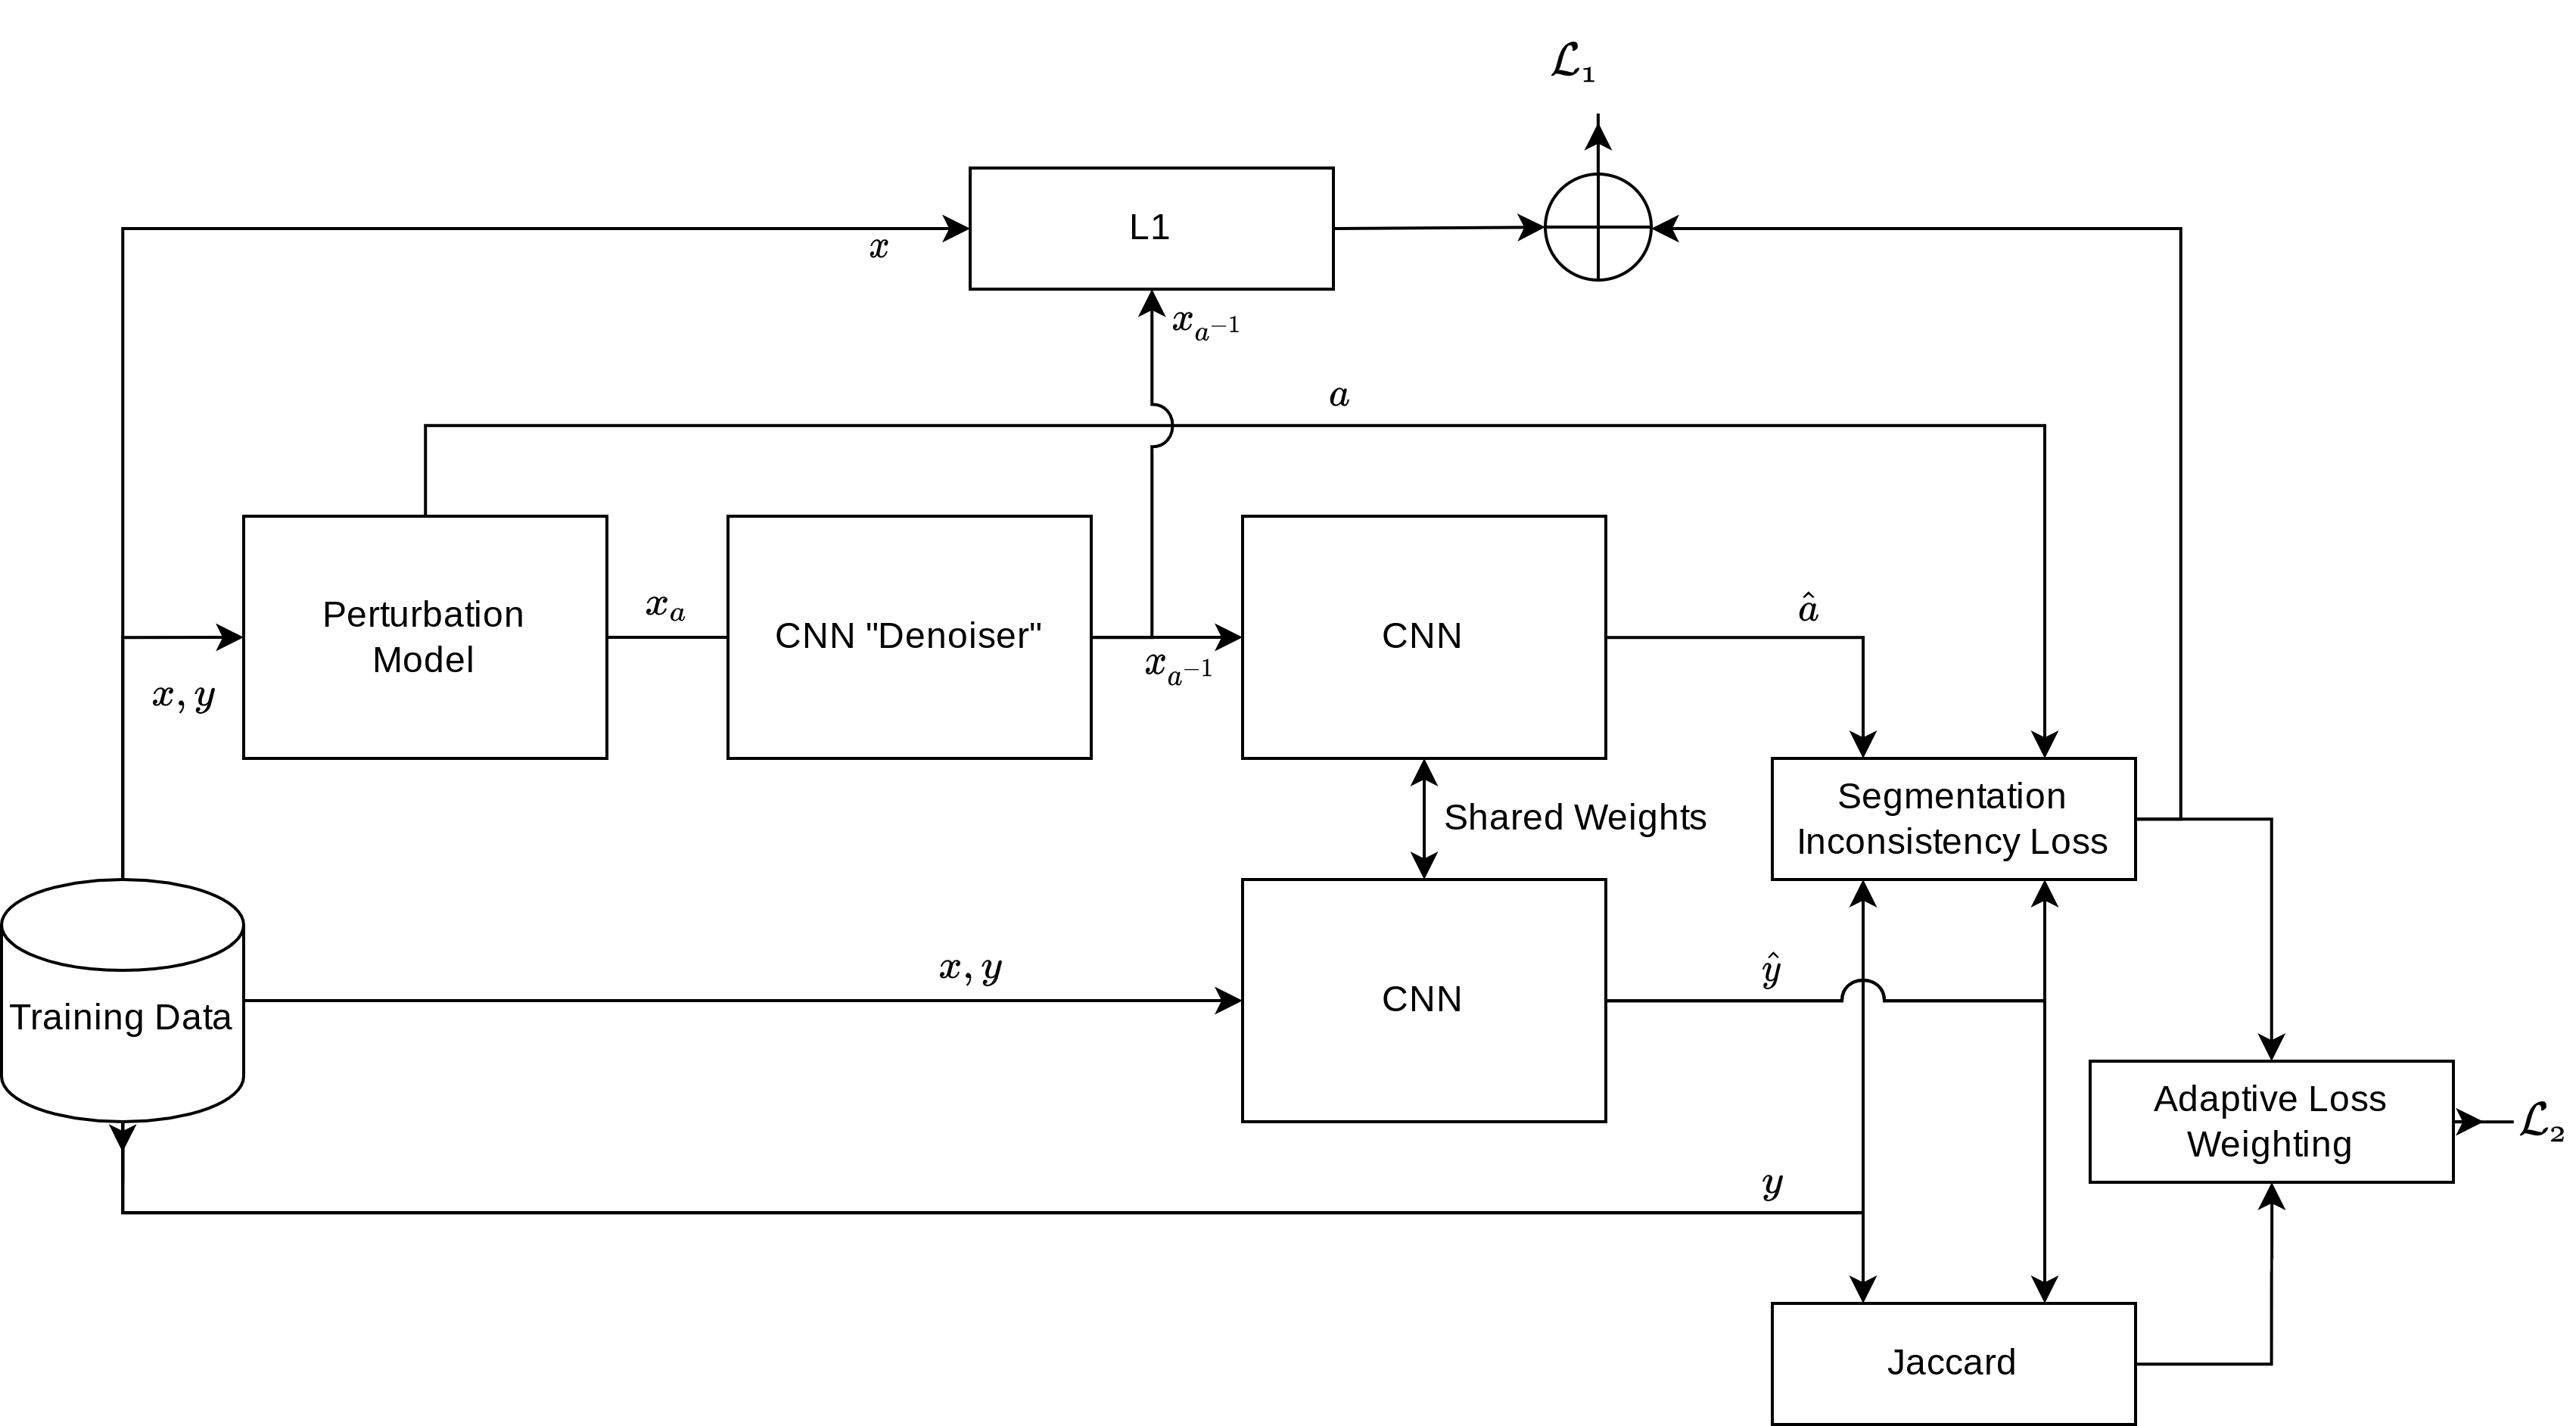
\includegraphics[width=\linewidth]{illustrations/deep_preprocessing.png}
            \caption{Consistency Preprocessing Pipeline}
            \label{fig:preproc}
        \end{figure}
        
        There are two main differences between this pipelines and more conventional deep denoising pipelines. First, the segmentation models are trained using Consistency Training. Second, the denoising network is incorporating inconsistency loss as a component of the loss function. There would in this case be two separate loss functions, one for each network. In theory, this should result in the denoiser learning to counteract the characteristics of the perturbations being applied that most negatively affect the consistency and thus the generalization of the segmentation models. Moreover, even if the denoiser performs poorly, the segmentation portion should be generalizable due to Consistency Training, which may even be improved as a result of whatever transforms the denoising network is performing.
        
        
    \subsection{Further investigations of multitask learning}
        Multitask learning was only briefly investigated in this thesis through the dual-decoder DeepLabV3+, which as a reminder performed image reconstruction as an auxiliary tasks. Though this was shown to have negligible effects, which was hypothesized may be the result of segmentation encoders learning task-agnostic features - the results are by no means sufficiently conclusive to discredit multitask learning altogether. 
    
        Further investigating the impact of multitask learning on generalization is as such warranted. One could for instance perform a study on the impact of different tasks; perhaps image reconstruction is less conducive to generalization than something more task-adjacent, such as dimming the background or simple object detection. Depending on the results of this study, one could then also experiment with adding multiple auxiliary tasks. Investigating the variance of the latent representation in these models across multiple runs of training and comparing these to the variance in single-task models may be interesting and further the understanding of what \glspl{dnn} actually learn.
        
        Modifying the models to a greater extent than merely adding additional decoders would in this case also be warranted. One may for instance investigate whether the segmentation task could be decoupled into a series of multiple stages consisting of simpler tasks.
    
    \subsection{Pretraining} \label{pretraining}
        A largely neglected but nevertheless impactful aspect of the deep learning pipelines studied in this thesis is the use of pretraining. Across all the experiments performed in this thesis, every predictor was pretrained on Imagenet, with the pretrained weights being included in the segmentation-models-pytorch library~\cite{smp}. Without pretraining, the models selected in this thesis exhibited \glspl{iou} of at best around 0.6 at best even on \gls{iid}, with even more significant performance gaps on \gls{ood} data. Naturally, non-pretrained networks are for this reason rarely used. However, this pretraining may play a key role in certain aspects of the behaviour observed in this thesis. In particular, pretraining may be the principle contributing factor behind the apparent ineffectiveness of multitask learning. An Imagenet pretrained encoder would, after all, perform the best when practically performing image compression.
        
            \subsection{Improving Ensembles through Diversity Search}
    Though ensembles as implemented in this thesis exhibit somewhat limited returns, leveraging a diversity of interpretations of the input data may have considerable merit towards increasing generalization. As the analysis in~\Cref{fig:ensemble_var} shows, there appears to be a positive relationship between generalizability and model-diversity that warrants further investigation. In particular, it may be the case that ensembles consisting of predictors that are trained to explicitly encode differing features are more conducive to generalization than conventionally implemented ensembles. By explicitly optimizing for weight diversity, one might mitigate the tendency of typical ensembles to primarily consider weight configurations that exhibit higher posterior likelihoods. 
    
    This could for instance be achieved by training multiple instances of the same model concurrently, and incorporating model-wise weight variance into the loss function. An illustration of such a pipeline is provided in~\Cref{fig:diversity}.
    
    \begin{figure}[htb]
        \centering
        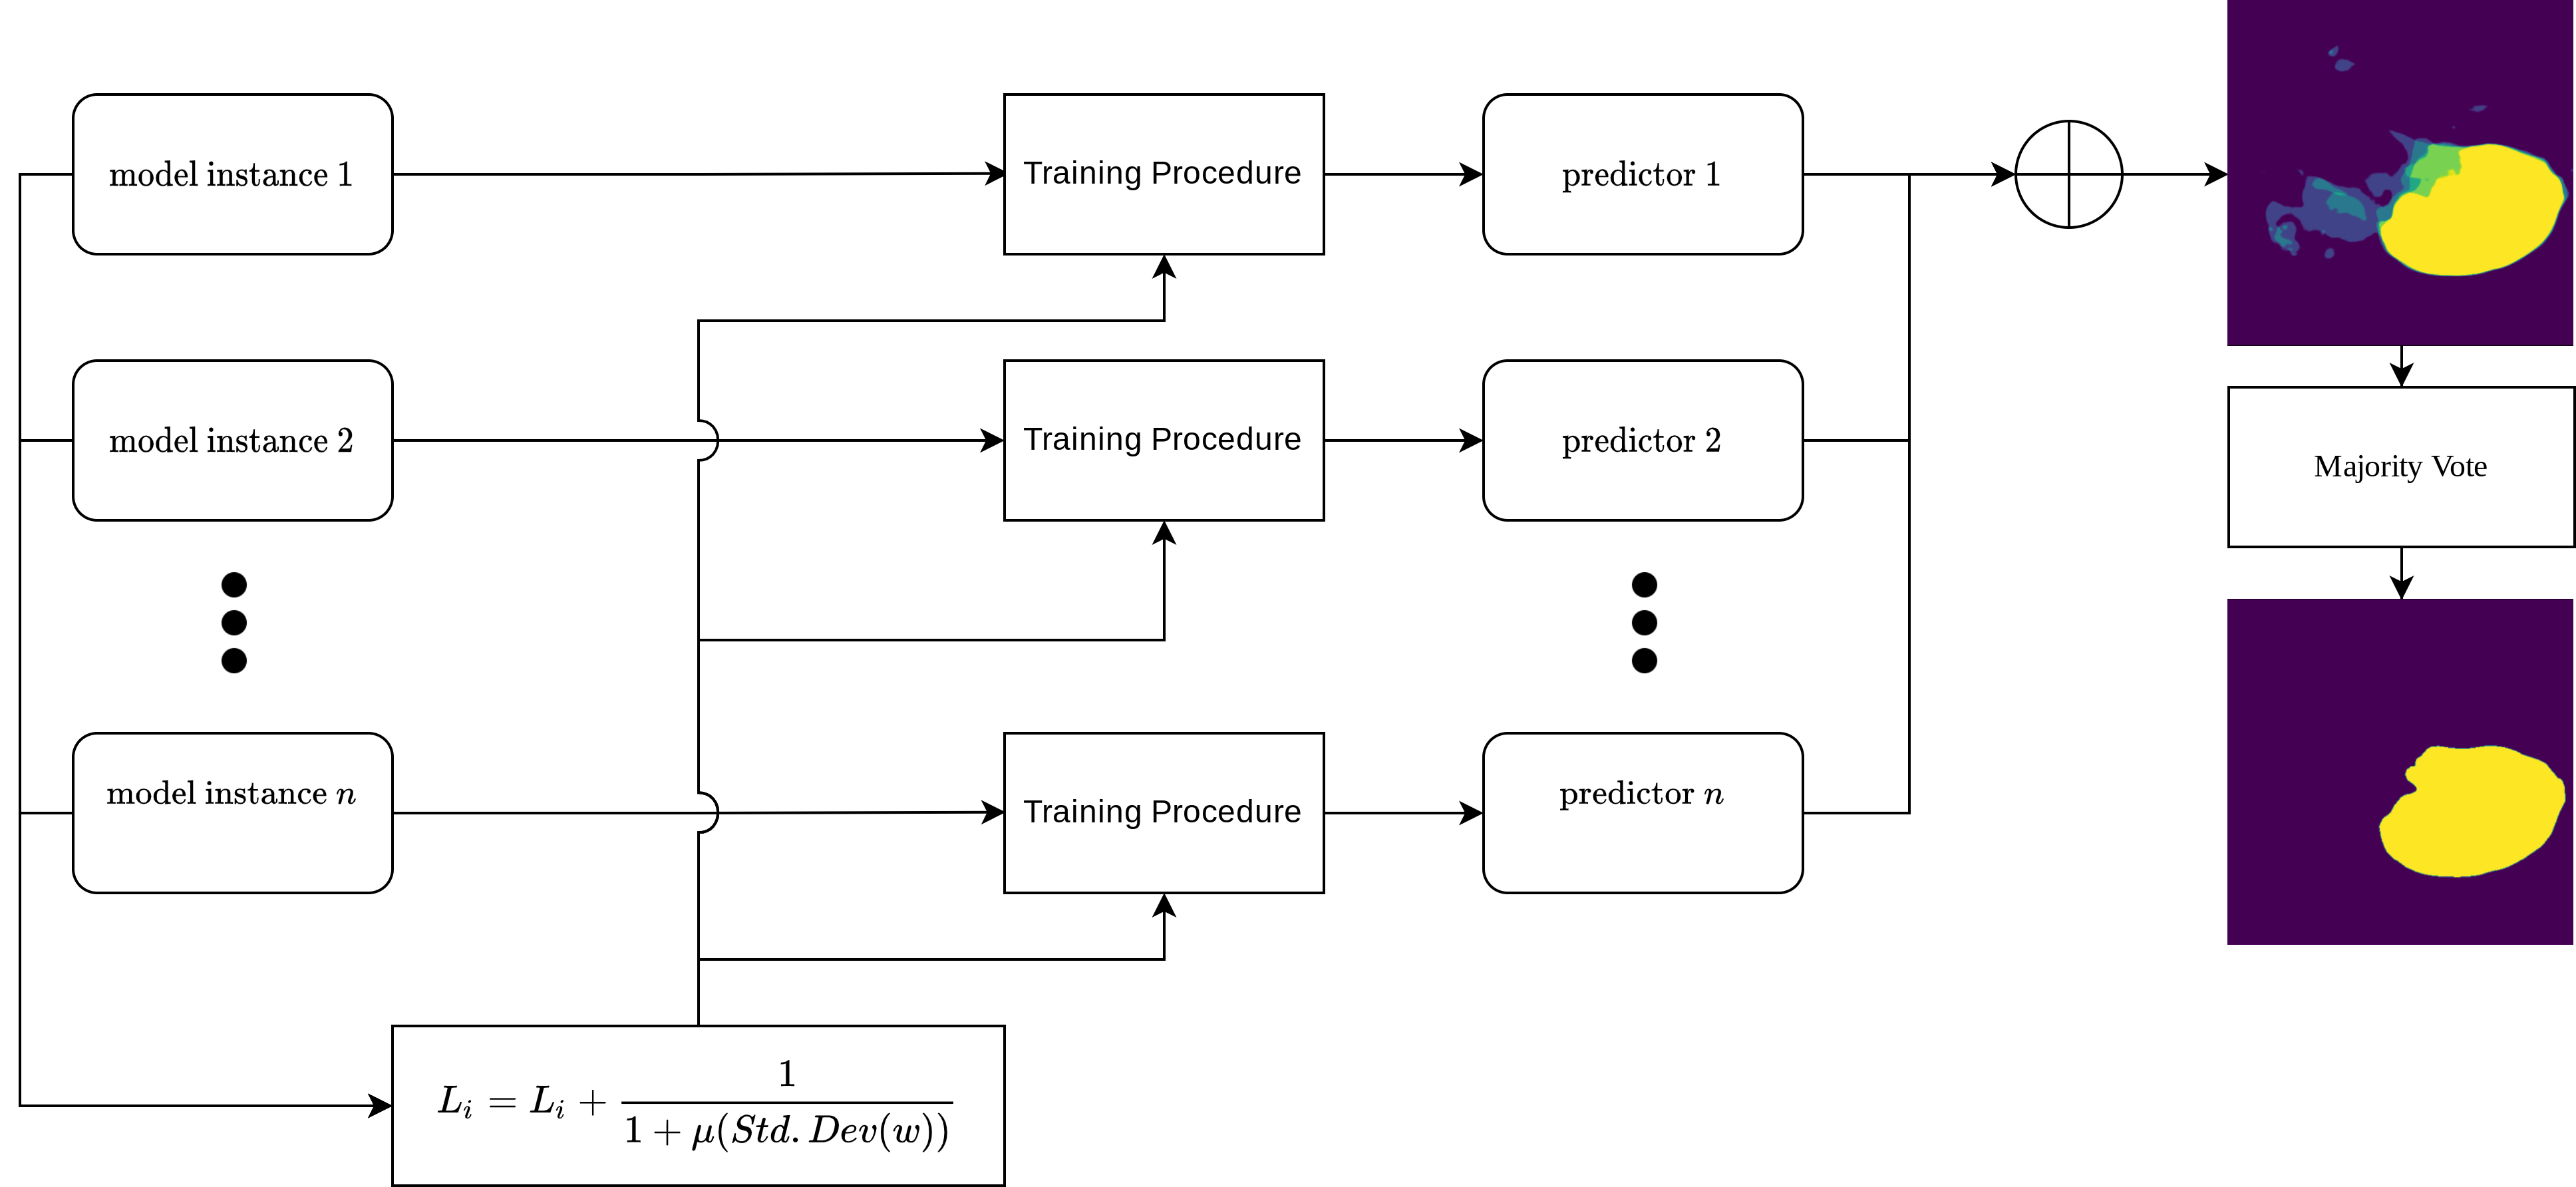
\includegraphics[width=\linewidth]{illustrations/diversity_search.png}
        \caption[Deep Diversity Search]{By adding a term corresponding to the mean standard deviation of weights, the models will learn maximally independent representations, and hence result in predictors with a larger diversity of learned features. This may mitigate underspecification to a greater extent, since this search would be less biased towards regions of the search landscape with high posterior probability.}
        \label{fig:diversity}
    \end{figure}
    
    This way, the ensemble will consist of predictors that encode a wider diversity of interpretations of the data than the predictors in conventional ensembles. This in turn provides a more complete perspective of the many possible interpretations a given model can learn. If this is proven to be the case, using such an ensemble during screening may also actually be viable, as the clinician could then take all of these possible interpretations into account instead of trusting that a single predictor is encoding the right inductive biases.  
